\chapter{Evaluation} \label{chap:Evaluation}
In diesem Kapitel sollen die Ergebnisse der angewendeten Methodik präsentiert werden. Des Weiteren wird eine Anforderungsanalyse durchgeführt, um zu beurteilen, welche Anforderungen umgesetzt wurden. Sollen einige nicht umsetzbar gewesen sein, so werden diese erläutert.

\section{Ergebnisevaluation der Vergleiche} \label{sec:Evaluation_Ergebnisevaluation}
In der Evaluation sollen die Ergebnisse, welche aus den Vergleichen stammten, präsentiert werden.

\subsection{Evaluation der Baseline Vergleiche}
Basierend auf dem Vorgehen \fullref{sec:Konzept_Vorgehen} wird mit den Baseline Vergleichen begonnen. Bei diesen handelt es sich um die Vergleiche, welche von  nicht optimierten Agenten (Baseline Agenten) durchgeführt worden sind \fullref{fig:Konzept_Agenten}). Diese Agenten wurden in einem Trainingsverlauf, entsprechend der Beschreibung im \autoref{subsec:Konzept_Datenerhebung}, trainiert. 
Währenddessen wurden die Trainingsdaten erhoben, die grafisch dargestellt wurden. 
Als nächster Schritt wurden die Testdaten ermittelt, welche im Folgenden tabellarisch ausgewertet werden mit Ausnahme der Robustheit und Effizienz. Bei diesen bietet sich eine grafische Auswertung der Testdaten an.

\subsubsection{Performance}
Die Baseline Vergleichsauswertung soll mit der Performance beginnen. Dabei ist in der \autoref{fig:Evaluation_Baseline_01_performance} die durchschnittliche Performance bzw. Apfelanzahl der letzten 200 Epochs pro Epoch abgebildet.\\
Die DQN Agenten waren in den Vergleichen nicht in der Lage, eine durchschnittliche Apfelsammelrate von 30 Äpfeln pro Spiel zu erreichen. 
Eine vermutliche Erklärung warum die Agenten des DQN Algorithmus keine guten Leistungen erzielen konnten, liegt in der Wahl von Zufallsaktionen. Die Komplexität des Spiels Snake steigt gegen Ende immer weiter an, da die Snake, mit zunehmenden Spielfortschritt, keine nicht zielführenden Schritte mehr gehen darf. In einer beengten Spielsituation könnte jeder falsche Schritt zum Tod führen, wobei durch zufällige Aktionen falsche Schritte durchgeführt werden könnten. Dadurch, dass das Spiel immer vorzeitig beendet würde, könnte der DQN Agent auch seine Leistung nicht weiter steigern, weil ihm die Daten zum Lernen fehlen würden.
\begin{figure}[H]
	\centering
	\includesvg[scale=0.4517]{baseline-performance}
	\caption[Baseline Vergleich Performance]{Baseline Vergleich der Performance für die Trainingsdaten. Die Performance ist als Apfelanzahl pro Epoch definiert. Für einen besseren Kurvenverlauf wird die durchschn. Performance der letzten 200 Epochs abgebildet.}
	\label{fig:Evaluation_Baseline_01_performance}
\end{figure}
Im Training konnten besonders die Leistungen der PPO Agenten PPO-03 und PPO-01 überzeugen. 
Der PPO-03 kann dabei besonders mit seinem schnellen Lernerfolg punkten, wohingegen der PPO-01 mit seiner annähernd linearen Stetigkeit überzeugen kann.
PPO-02 konnte zwar ebenfalls ein fast lineare Steigerung seiner Performance erzielen, jedoch konvergierte dieser früher als der PPO-01.
Dieses Verhalten der Agenten entspricht den Darstellungen im \autoref{subsec:Konzept_Vorstellung_Agenten}.
\begin{longtable}[h]{|p{2.7cm}|p{4.5cm}|p{4cm}|}
	\hline
	Agent & Gemittelte Performance & Standardabweichung \\
	\hline
	DQN-01 & 17.7812 & 2.9577 \\
	\hline
	DQN-02 & 26.4226 & 4.3482 \\
	\hline
	DQN-03 & 25.4506 & 4.8280 \\
	\hline
	PPO-01 & 44.4544 & 19.6957 \\
	\hline
	PPO-02 & 38.7325 & 11.5756 \\
	\hline
	PPO-03 & 46.4268 & 14.0280 \\
	\hline
\caption{Testdatenauswertung der Performance}
\label{tab:Evaluation_Testdaten_Performance} 
\end{longtable}
\newpage
Auch die Auswertung der Testdaten \fullref{tab:Evaluation_Testdaten_Performance} zeigt den sich in den Trainingsdaten abzeichnenden Trend. So erbringt der PPO-03 die beste und der PPO-01 die zweitbeste Leistung. Die Standardabweichungen des PPO-03 und PPO-01 zeigen jedoch, dass die Leistungen nicht konsistent sind. Besonders PPO-01 zeigte eine schwankende Performance, welche auch in den Trainingsdaten \fullref{fig:Evaluation_Baseline_01_performance} zu beobachten ist.
Daher bleibt der PPO-03 für das Evaluationskriterium der Performance der Sieger.\\
Stark mit der Performance korrelierend, stellt die Siegrate das nächste zu untersuchende Evaluationskriterium dar.

\subsubsection{Siegrate} \label{sec:Evaluation_Siegrate}
Ähnlich wie bei der Performance verhält es auch mit dem Evaluationskriterium der Siegrate. PPO-03 und PPO-01 besitzen die besten Siegraten während des Trainings \fullref{fig:Baseline_winrate}.
\begin{figure}[H]
	\centering
	\includesvg[scale=0.4517]{baseline-siegrate}
	\caption[Baseline Vergleich Siegrate]{Baseline Vergleich der durchschn. Siegrate. Für den besseren Kurvenverlauf wird die durchschn. Siegrate der letzten 200 Epochs abgebildet.}
	\label{fig:Baseline_winrate}
\end{figure}
Die DQN Agenten sind nicht in der Lage gewesen Siege zu erreichen und fallen daher aus der Betrachtung heraus.
Der PPO-02 zeigt eine deutlich geringe Siegrate, trotz ähnlicher Performances zu den anderen PPO Agenten.
Bemerkenswert ist des Weiteren, dass der PPO-03 zwar ähnliche Leistungen wie der PPO-01 erreicht \fullref{fig:Evaluation_Baseline_01_performance}, jedoch der PPO-01 eine deutlich bessere Siegraten erzielt. Dies ist möglicherweise auf den stetigen Lerncharakter des Agenten zurückzuführen \fullref{subsec:Konzept_Vorstellung_Agenten}.
Auch die Testdaten in \autoref{tab:Evaluation_Testdaten_Winrate} zeigen, dass PPO-01 der Sieger ist, wobei sich der eben beschriebene Trend aus den Trainingsdaten in den Testdaten widerspiegelt. Daher ist der PPO-01 der Sieger für das Evaluationskriterium der Siegrate.
\newpage
\begin{longtable}[h]{|p{3.7cm}|p{4.5cm}|p{4.5cm}|}
	\hline
	Agent & Gemittelte Siegraten & Standardabweichung \\
	\hline
	PPO-01 & 0.6759 & 0.33306 \\
	\hline
	PPO-02 & 0.0926 & 0.20478 \\
	\hline
	PPO-03 & 0.3316 & 0.32751 \\
	\hline
	\caption{Testdatenauswertung der Baseline Siegrate}
	\label{tab:Evaluation_Testdaten_Winrate} 
\end{longtable}
\subsubsection{Robustheit}
Die Robustheit stellt ein besonderes Evaluationskriterium dar, denn sie wird ausschließlich aus Testdaten bestimmt. Diese werden zur besseren Übersicht in eine Grafik überführt. Die Robustheit ist als durchschn. Apfelanzahl dividiert durch die Spielfeldgröße pro Quadratwurzel aus der Spielfeldgröße definiert. 
\begin{figure}[H]
	\centering
	\includesvg[scale=0.4517]{baseline-robustheit}
	\caption[Baseline Vergleich Robustheit]{Baseline Vergleich der durchschn. Robustheit. Diese wird als durchschn. Apfelanzahl dividiert durch die Spielfeldgröße pro Quadratwurzel aus der Spielfeldgröße dargestellt.}
	\label{fig:Evaluation_Baseline_Robustheit}
\end{figure}
Wie in \autoref{fig:Evaluation_Baseline_Robustheit} zu erkennen ist, zeigen die DQN Agenten keine guten Resultate.
Sie erreichen auf kleineren Spielfeldgrößen bessere Ergebnisse als auf der Standard Spielfeldgröße von 8x8. Sollte sich jedoch das Spielfeld vergrößern, so stagnieren ihre Leistungen.
Bei den PPO Agenten zeigt sich ein ähnliches Bild. Ihre Leistungen steigen ebenfalls nicht mit dem sich vergrößernden Spielfeld an. Jedoch ist der PPO-03 in der Lage, die besten Ergebnisse in den unbekannten Gebieten zu erzielen.\\
Bemerkenswert ist des Weiteren, dass sich ein Trend abzeichnet, nachdem Agenten auf geraden Spielfeldgrößen (z.B. (6x6), (8x8) und (10x10)) bessere Leistungen erzielen können als auf ungeraden (z.B. (7x7) und (9x9)).\\
Aus diesem Vergleich geht dennoch der PPO-03 Agent als Sieger für das Evaluationskriterium der Robustheit hervor.

\subsubsection{Effizienz} \label{sec:Evaluation_Effizienz_Baseline}
Die Effizienz stellt zusammen mit der Robustheit ein besonderes Evaluationskriterium dar. Sie ist als durchschn. Schrittanzahl pro Apfelanzahl definiert.\\
Wie in der \autoref{fig:Evaluation_Baseline_Effizienz} zu erkennen ist, sind DQN-01 und DQN-02 diejenigen, welche die niedrigste Schrittanzahl für die jeweilige Apfelanzahl besitzt. Dies gilt jedoch nicht kontinuierlich. Denkbar wären daher die DQN Agenten in Einsatzgebieten mit wenigen Zielen aber großen Distanzen einzusetzen, sodass der Effizienzcharakter der Agenten hilft Kraftstoff bzw. Energie, am Beispiel der unbemannten Drohnen, zu sparen. 
\begin{figure}[H]
	\centering
	\includesvg[scale=0.4517]{baseline-effizienz}
	\caption[Baseline Vergleich der Effizienz für die Trainingsdaten]{Baseline Vergleich der Effizienz für die Trainingsdaten. Die Effizienz ist als durchschn. Schrittanzahl pro Apfelanzahl dargestellt.}
	\label{fig:Evaluation_Baseline_Effizienz}
\end{figure}
Eine weitere Betrachtung der DQN Agenten unter dem Kriterium der Effizienz wird jedoch aufgrund der fehlenden Daten nicht durchgeführt.
Da die DQN Agenten ausgeschieden sind, bleiben nur noch die PPO Agenten. Diese verfügen über den gesamten Trainingslauf eine solide Effizienz.
Der PPO-02 konnte bei der Auswertung der Trainingsdaten die besten Ergebnisse erzielen, gefolgt von PPO-03.
Erwähnenswert ist ebenfalls, dass das die Effizient-Differenz zwischen den Agenten PPO-01 bis PPO-03 gegeben Ende deutlich abnimmt, da durch die Gesetzmäßigkeiten des Spiels Snake, kaum effizientere Routen zum Apfel zu finden sind.
Auch bei der Auswertung der Testdaten in Abbildung \ref{fig:Evaluation_Effizienz2_Baseline}, wird dieser Trend deutlich.\\
Einzelnen Graphen in Abbildung \ref{fig:Evaluation_Effizienz2_Baseline} besitzen immer wieder Abschnitte, in welchen der Graph abbricht. Dies bedeutet, dass der Agent eine solche Anzahl an Äpfeln nie erreicht hat. Dies muss nicht negativ ausgewertet werde.\\
Die gute Effizienz des PPO-02 kann dabei unter anderen auf den niedrigen Gamma Wert von 0.93 zurückgeführt werden, welcher den Agenten dazu anhält, schnell viele gute Rewards zu erzielen (siehe Abschnitt \ref{sec:Konzept_Vorstellung_Agenten}).
\begin{figure}[H]
	\centering
	\includesvg[scale=0.4517]{baseline-effizienz2}
	\caption[Baseline Vergleich der Effizienz für die Testdaten]{Baseline Vergleich der Effizienz - Testdaten}
	\label{fig:Evaluation_Effizienz2_Baseline}
\end{figure}

\subsection{Evaluation der Optimized Vergleiche}
Nach der Durchführung der Baseline Vergleiche werden nun, entsprechend des Vorgehens (siehe Abschnitt \ref{sec:Konzept_Vorgehen}), die Baseline Gewinner Agenten (siehe Abbildung \ref{fig:Vorgehen}) optimiert und dann untereinander verglichen.
Dabei ist es auch möglich, sofern sich die Optimierungen nicht gegenseitig ausschließen, die Agenten mit mehr als nur einer Optimierung als zusätzlichen Parameter auszustatten. Dies wird jedoch in dieser Ausarbeitung, trotz der bestehenden Möglichkeit, nicht durchgeführt, um damit die Menge an Agenten nicht zu stark auszuweiten. Dies schafft eine bessere Übersichtlichkeit bei den Auswertungen.\\
Ebenfalls werden die Gewinner der Baseline Vergleiche mit in die Optimized Vergleiche eingebunden. Die Ergebnisse finden sich in den Folgenden Abschnitten.

\subsubsection{Performance} \label{sec:Evaluation_Performance_Optimized}
\begin{figure}[H]
	\centering
	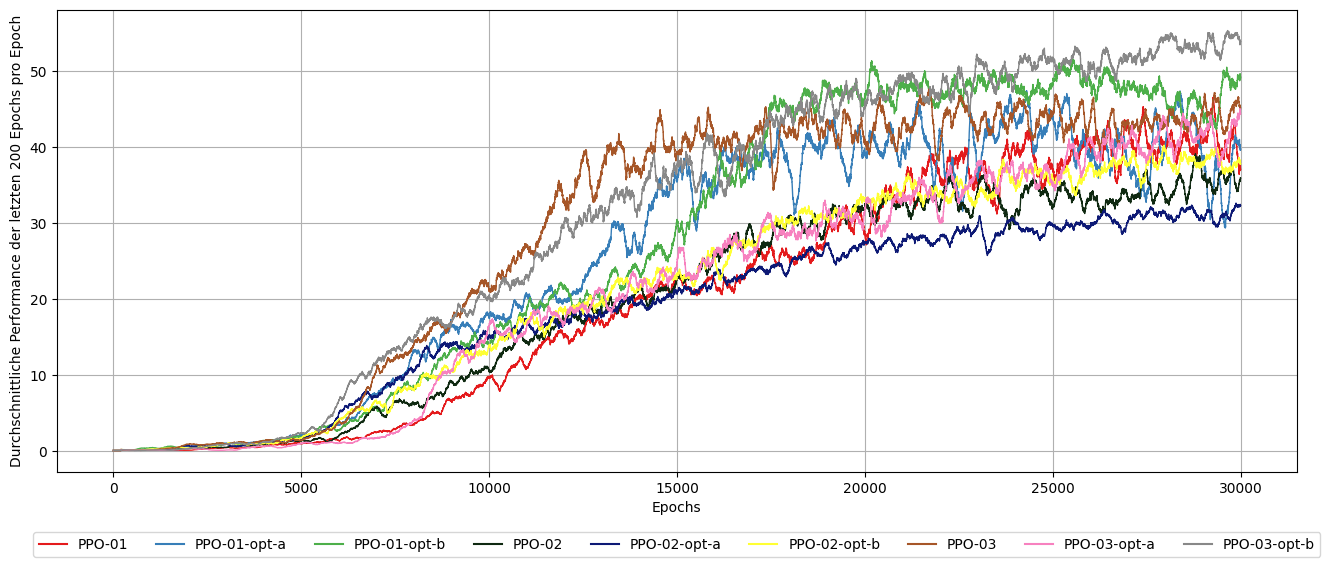
\includegraphics[scale=0.4517]{Abbildungen/Evaluation/optimized-performance.png}
	\caption[Optimized Vergleich Performance]{Baseline Vergleich eins (oben) und zwei (unten) der Effizienz}
	\label{fig:Optimized_Performance}
\end{figure}
Wie in Abbildung \ref{fig:Optimized_Performance} zu erkennen ist, sind die Leistungen der einzelnen Agenten sehr unterschiedlich. Alle Agenten, welche auf dem PPO-02 aufbauen (Dunkelgrün, Dunkelblau und Gelb), konnten sich in diesem Vergleich nicht behaupten und schnitten schlechter als alle anderen Agenten ab. Dies könnte mit der Kurzzeitpräferenz, ausgelöst durch den niedrigen Gamma Wert, in Verbindung stehen. Die Ergebnisse der PPO-01 Agenten (Rot, Hellblau, Hellgrün) liegen im Mittelfeld, mit Ausnahme des PPO-01-opt-b, welcher das zweit beste Ergebnis erzielen konnte. Im oberen Mittelfeld sind die Agenten, welche von PPO-03 abstammen. Diese beinhalten auch den Gewinner bezüglich der Trainingsdaten. PPO-03-opt-b konnte seine Leistungen in den letzten 5.000 Trainingsspielen noch verbessern, im Gegensatz zum PPO-01-opt-b.\\
Insgesamt schnitten die Agenten mit der Optimierung B immer besser ab als die mit der Optimierung A (PPO-01-opt-a, PPO-02-opt-a, PPO-03-opt-a) und die nicht optimierten (PPO-01, PPO-02, PPO-03). Optimierung A stellte sich unter dem Gesichtspunkt der Performancesteigerung sogar als hinderlich heraus, da die Leistungen der optimierten Agenten entweder ungefähr gleich blieben (siehe die Agenten von PPO-01 und PPO-03) oder schlechter wurden (siehe die Agenten von PPO-02).
\begin{longtable}[h]{|p{3.2cm}|p{6cm}|p{4cm}|}
	\hline
	Agent & Durchschnittliche Performance & Standardabweichung \\
	\hline
	PPO-01 & 44.4544 & 19.6957 \\ 
	\hline
	PPO-01-opt-a & 45.8125 & 18.1183 \\ 
	\hline
	PPO-01-opt-b & 45.6213 & 18.7242 \\ 
	\hline
	PPO-02 & 38.7325 & 11.5756 \\ 
	\hline
	PPO-02-opt-a & 34.8827 & 6.9273 \\ 
	\hline
	PPO-02-opt-b & 42.5969 & 12.4416 \\ 
	\hline
	PPO-03 & 46.4268 & 14.0280 \\ 
	\hline
	PPO-03-opt-a & 48.7674 & 14.9580 \\ 
	\hline
	PPO-03-opt-b & 56.1117 & 12.3773 \\ 
	\hline
	\caption{Testdatenauswertung der Performance}
	\label{tab:Evaluation_Testdaten_Performance_Optimized} 
\end{longtable}
Auch die Testdaten (siehe Tabelle \ref{tab:Evaluation_Testdaten_Performance_Optimized}) geht hervor, dass der PPO-03-opt-b der Sieger dieses Vergleiches ist. Mit einer Standardabweichung, welche sich insgesamt im Mittelfeld befindet (siehe Tabelle \ref{tab:Evaluation_Testdaten_Performance_Optimized}), von 12.3773 zeigt sich jedoch, das der PPO-03-opt-b dieser Leistung nicht kontinuierlich erzielen kann. Jedoch bleibt der PPO-03-opt-b, selbst unter Einbeziehung der Standardabweichung der Gewinner im Evaluationskriterium der Performance.\\
Als nächsten Evaluationskriterium wird die Sieg-Rate, entsprechend der Priorisierung (siehe Abschnitt \ref{sec:Konzept_Vorgehen}), thematisiert.

\subsubsection{Siegrate} \label{sec:Evaluation_Siegrate_Optimized}
Die Sieg-Rate spiegelt ein ähnliches Bild wieder wie bei der zuvor thematisierten Performance (siehe Abschnitt \ref{sec:Evaluation_Performance_Optimized}). Der PPO-03-opt-b konnte auch hier bei den Trainingsdaten die besten Ergebnisse zeigen. 
\begin{figure}[H]
	\centering
	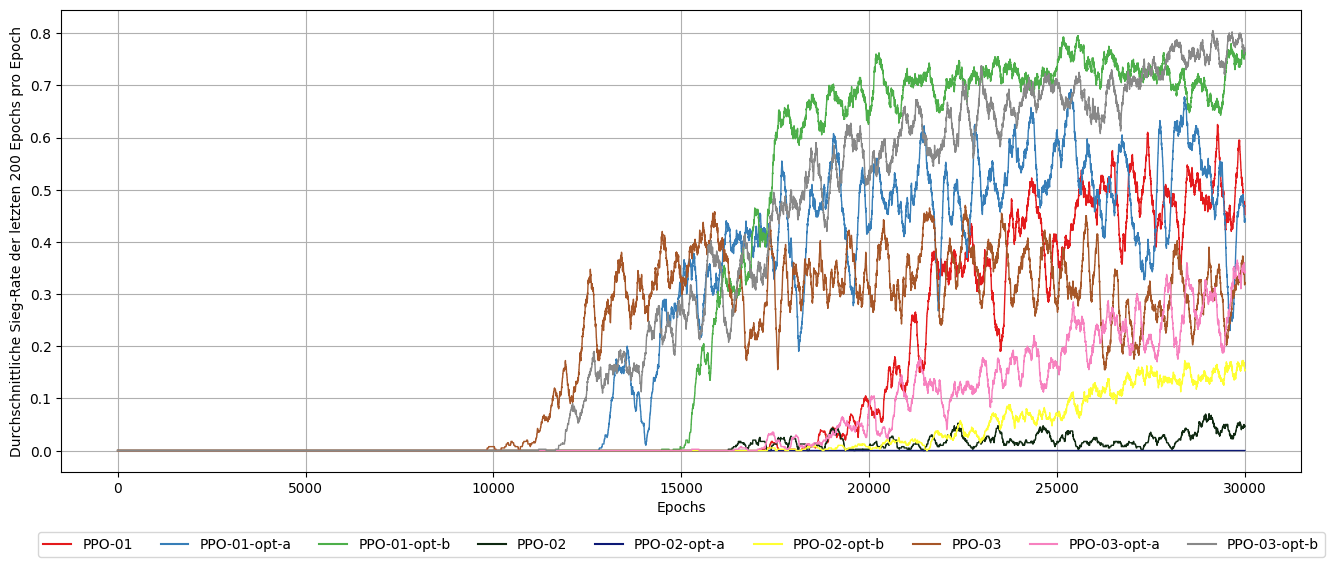
\includegraphics[scale=0.4517]{Abbildungen/Evaluation/optimized-winrate.png}
	\caption[Optimized Vergleich Siegrate]{Optimized Vergleich eins (oben) und zwei (unten) der Siegrate}
	\label{fig:Optimized_Winrate}
\end{figure}
Die PPO-02 Agenten konnten wieder keine guten Leistungen erreichen. Interessant ist die Tatsache, dass die PPO-03 Agenten, mit Ausnahme des PPO-03-opt-b, bei den Sieg-Raten eher im unteren Mittelfeld liegen und die Sieg-Raten der PPO-01 Agenten, mit Ausnahme des PPO-01-opt-b, im oberen Mittelfeld. Dies stellt einen gegensätzliches Verhalten zur Performance dar.
Wie die Auswertung der Testdaten (siehe Tabelle \ref{tab:Evaluation_Testdaten_Winrate_Optimized}) zeigt, ist der PPO-03-opt-b auch hier der gesamt Sieger. Mit einer Sieg-Rate von 0.8466 übertrifft er selbst den Zweitplatzierten PPO-01-opt-b, welcher nur eine Sieg-Rate von 0.7186 erreichte.
\begin{longtable}[h]{|p{3.2cm}|p{6cm}|p{4cm}|}
	\hline
	Agent & Durchschnittliche Sieg-Rate & Standardabweichung \\
	\hline
	PPO-01 & 0.6759 & 0.3331 \\ 
	\hline
	PPO-01-opt-a & 0.6551 & 0.3377 \\ 
	\hline
	PPO-01-opt-b & 0.7186 & 0.3011 \\ 
	\hline
	PPO-02 & 0.0926 & 0.2048 \\ 
	\hline
	PPO-02-opt-a & 0.0001 & 0.0071 \\ 
	\hline
	PPO-02-opt-b & 0.2354 & 0.2496 \\ 
	\hline
	PPO-03 & 0.3316 & 0.3275 \\ 
	\hline
	PPO-03-opt-a & 0.5273 & 0.3479 \\ 
	\hline
	PPO-03-opt-b & 0.8466 & 0.2482 \\ 
	\hline
	\caption{Testdatenauswertung der Optimized Sieg-Raten}
	\label{tab:Evaluation_Testdaten_Winrate_Optimized} 
\end{longtable}
Damit ist der PPO-03-opt-b der Sieger des Evaluationskriteriums der Sieg-Rate. Als nächstes folge die Betrachtung der Robustheit, entsprechend der Priorisierung (siehe Abschnitt \ref{sec:Konzept_Vorgehen}).

\subsubsection{Robustheit}
\begin{figure}[H]
	\centering
	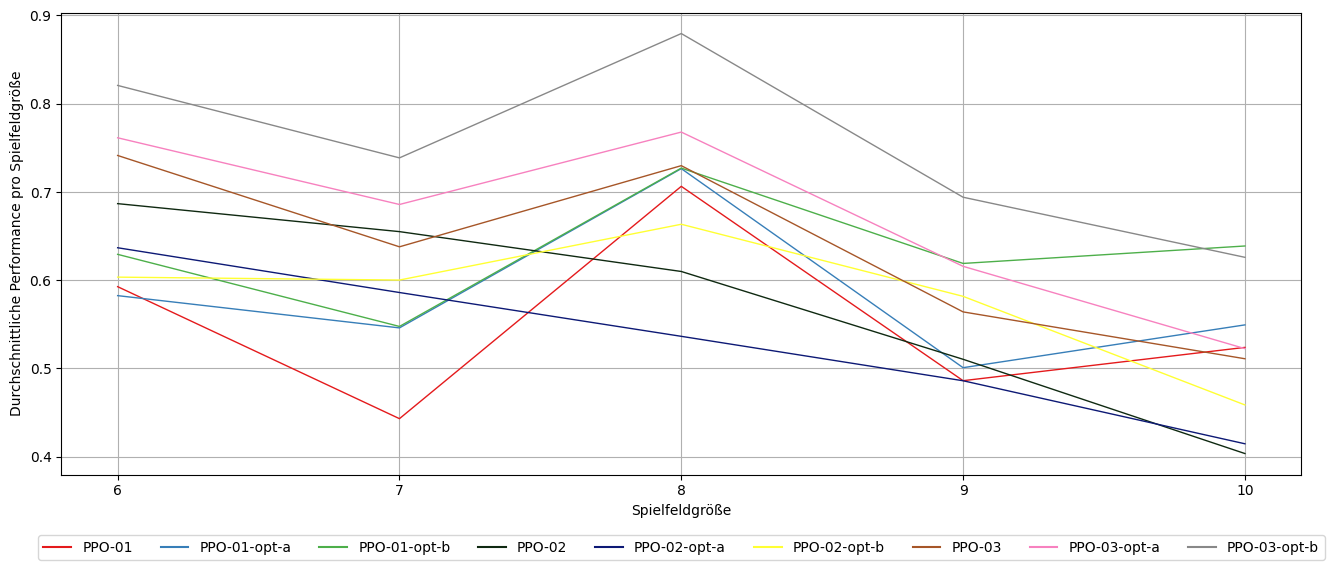
\includegraphics[scale=0.4517]{Abbildungen/Evaluation/optimized-robustheit.png}
	\caption[Optimized Vergleich Siegrate]{Optimized Vergleich eins (oben) und zwei (unten) der Siegrate}
	\label{fig:Evaluation_Robustheit_Optimized}
\end{figure}
Nach der Testauswertung (siehe Abbildung \ref{fig:Evaluation_Robustheit_Optimized}) hat sich der PPO-03-opt-b als der robusteste Agent dargestellt.
Dabei zeigt die Abbildung \ref{fig:Evaluation_Robustheit_Optimized} die durchschnittliche Performance für jede Spielfeldgröße.
Von allen Agenten wies er die kontinuierlichste Performance vor. Sowohl auf größeren als auch auf kleineren Spielfeldern zeigt er eine gute Leistung und damit eine solide Robustheit.\\
Es ist daher festzuhalten, dass der PPO-03-opt-b der Sieger für das Evaluationskriterium der Robustheit ist.
Interessant ist des Weiteren, dass die Leistungen auf ungeraden Spielfeldgrößen (7, 9) nicht so gut ist, wie auf geraden Spielfeldgrößen (6, 8, 10). Es kann daher angenommen werden, dass die Strategie der Agenten in irgendeiner Form von der Spielfeldgröße abhängig ist, obwohl diese dem Agenten nicht in der Observation direkt übergeben wird (siehe Abschnitt \ref{sec:Konzept_Observation}).

\subsubsection{Effizienz}
Die Abbildung \ref{fig:Evaluation_Effizienz_Optimized} zeigt die durchschnittliche Schrittanzahl der einzelnen Agenten für jede Apfelanzahl. Die Effizienz ist dabei als Schritte pro Apfel definiert. Wie in Abbildung \ref{fig:Evaluation_Effizienz_Optimized}zu erkennen ist, benötigt der PPO-02-opt-a die wenigsten Schritte um die dargelegte Anzahl an Äpfeln zu sammeln. Dieser scheidet jedoch aufgrund seiner unzureichenden Daten aus. Der Sieger der Trainingsdaten ist damit der PPO-03-opt-a, gefolgt von dem PPO-03-opt-b. Insgesamt ist jedoch zu bemerken, dass alle Agenten ähnliche Effizienzen zeigen.
\begin{figure}[H]
	\centering
	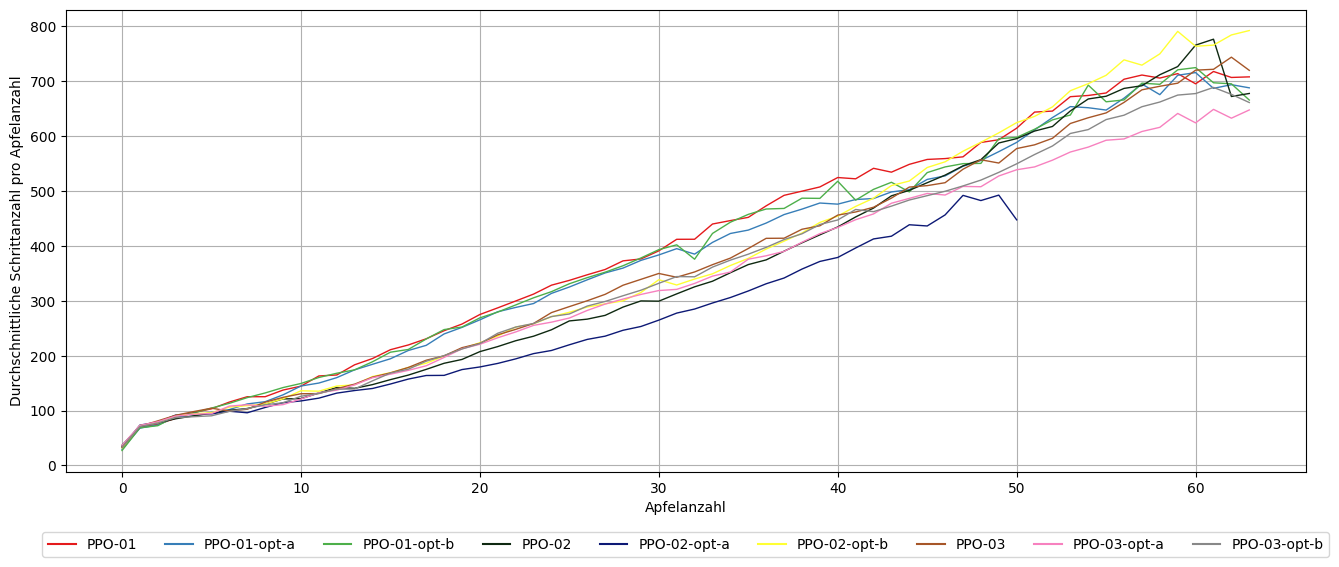
\includegraphics[scale=0.4517]{Abbildungen/Evaluation/optimized-effizienz.png}
	\caption[Optimized Vergleich Effizienz]{Optimized Vergleich der Effizienz - Trainingsdaten}
	\label{fig:Evaluation_Effizienz_Optimized}
\end{figure}
Die Auswertung der Testdaten zeigt ein ähnliches Bild (siehe Abbildung \ref{fig:Evaluation_Effizienz2_Optimized}). Auch hier erweist sich der PPO-03-opt-a als der effizienteste, gefolgt von dem PPO-03-opt-b.\\
Wie bereits in Abschnitt \ref{sec:Evaluation_Effizienz_Baseline} erwähnt, besitzen die einzelnen Graphen immer wieder Abschnitte, in welchen der Graph abbricht. Dies bedeutet, dass der Agent eine solche Anzahl an Äpfeln nie erreicht hat.
\begin{figure}[H]
	\centering
	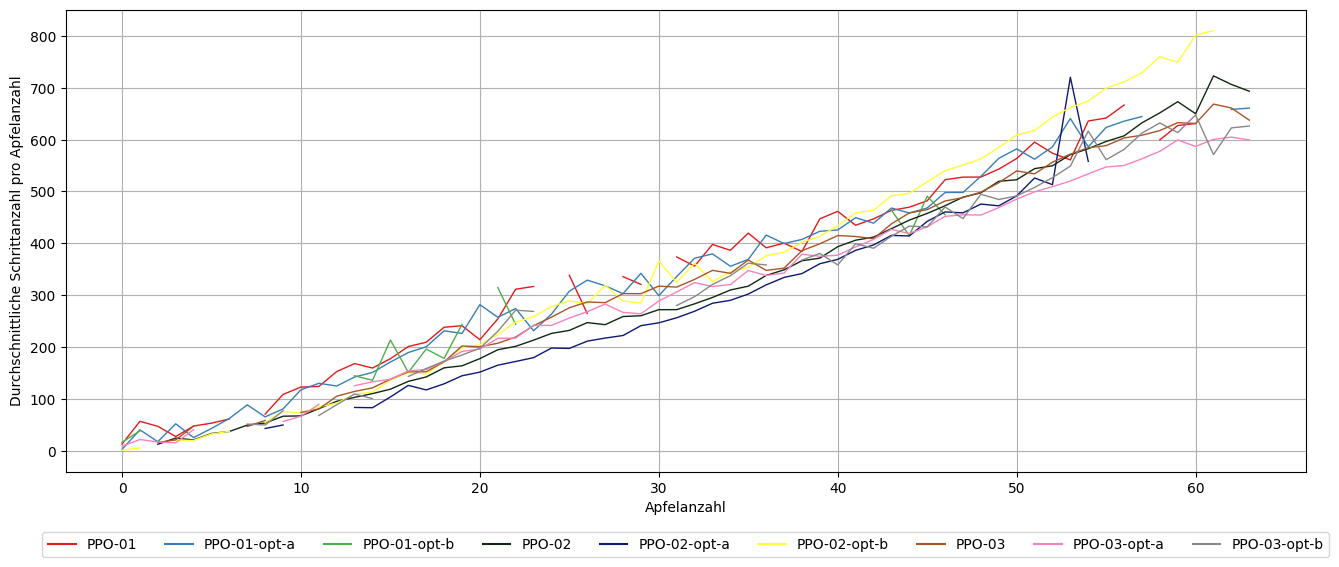
\includegraphics[scale=0.4517]{Abbildungen/Evaluation/optimized-effizienz2.png}
	\caption[Optimized Vergleich Effizienz]{Optimized Vergleich der Effizienz - Testdaten}
	\label{fig:Evaluation_Effizienz2_Optimized}
\end{figure}
Der Sieger dieses letzten Vergleichs ist der PPO-03-opt-a.

\subsection{Bestimmung des optimalen Agenten}
In diesem Abschnitt soll  nun der optimale Agent ermittelt werde. Basierend auf den Ergebnissen der Vergleiche stellt sich heraus, dass der PPO-03-opt-b Agent der optimale Agent ist. Er liefert die besten Resultate in den Evaluationskriterien der Performance, Sieg-Rate und Robustheit. Einzig in der Effizienz belegt er den zweiten Platz. Basierend auf der Priorisierung (siehe Abschnitt \ref{sec:Konzept_Vorgehen}) ist damit der PPO-03-opt-b der gesamt Sieger.


\section{Anforderungsevaluation}
Zu Beginn sollen die Anforderungen an das Environment evaluiert werden. Danach folgen die Evaluationen der Anforderungen Agenten und der Datenerhebung. Zum Schluss sollen evaluiert werden, ob alle Anforderungen bezüglich der Statistiken und der Evaluation selbst erfüllt worden sind.

\subsection{Anforderungsevaluation der Environment}
Die Hauptanforderung an das Env besagt, dass das Spiel Snake implementiert werden soll. Im Rahmen dieser Ausarbeitung wurde das Spiel Snake nach der Beschreibung in Anschnitt \ref{sec:Grundlagen_Game_of_Snake} implementiert. Diese Anforderung kann daher als erfüllt angesehen werden. Eine Darstellung der Implementierung findet sich im Abschnitt des Konzepts (siehe Abschnitt \ref{sec:Konzept_Environment}) und in der Implementierung (siehe Abschnitt \ref{sec:Implementierung_Environment}).\\
\\ Ebenfalls wurde die Anforderung der Standardisierten Schnittstelle (siehe Abschnitt \ref{sec:Anforderungen_Schnittstelle}), welche zu einer Normung und damit zu einer einfacheren Benutzung des Environment führen soll, erfüllt. Wie in dem Abschnitt \ref{sec:Konzept_Schnittstelle} und \ref{sec:Implementierung_train_Methode} zu sehen ist, werden Aktionen, durch die step Methoden entgegengenommen, Rewards und Observationen zurückgegeben. Neben der step Methode wird die Observation auch noch durch die Schnittstellenmethode reset geliefert. Diese beiden Methoden spannen die standardisierte Schnittstelle auf.\\
\\ Auch sind die funktionalen Anforderungen, welche den geregelten Ablauf im Environment garantieren, beachtet worden.
So wird die Aktionsausführung (siehe Abschnitt \ref{sec:Anforderungen_Aktionsausführung}) durch die action Methode in der SnakeGame Klasse durchgeführt, welche von der Schnittstellenmethode step aufgerufen wird. Die reset und render Anforderungen (siehe Abschnitte \ref{sec:Anforderung_Reset} und \ref{sec:visualisierung_Env}) werden durch die gleichnamigen Schnittstellenmethode abgedeckt (siehe Abschnitte \ref{sec:Konzept_Spielablauf} und \ref{sec:Implementierung_Environment}).

\subsection{Anforderungsevaluation der Agenten}
Der nächste großer Anforderungsbereich behandelt die Agenten. Zu diesem Zweck wurden die Anforderungen der Aktionsbestimmung und des Lernens aufgestellt. Diese stellen die grundlegenden Funktionen der Agenten dar. 
Wie im Konzept dargestellt ist, wurde sowohl der DQN als auch der PPO Agent mit einer Aktionsauswahlmethode (siehe Abschnitte \ref{sec:Implementierung_act_PPO} und \ref{sec:Implementierung_act_DQN}) und einer learn Methode (siehe Abschnitte \ref{sec:Implementierung_learn_DQN} und \ref{sec:Implementierung_learn_PPO}) ausgestattet. Diese implementieren das geforderte Verhalten aus den Anforderungen (siehe Abschnitt \ref{sec:Agent_Funktionalitäten}).\\
\\Neben den funktionalen, existieren noch zwei weitere Anforderungen. Zu diesen gehört die Diversität der Algorithmen (siehe Abschnitt \ref{sec:Anforderungen_Diversität}).\\
Diese fordert den Vergleich verschiedener Algorithmen und dabei insbesondere des PPO und DQN Algorithmus. Mit dieser Forderung kann die entwickelte Methodik (siehe Abschnitt \ref{sec:Konzept_Vorgehen}) besser bewertet werden. Diese Anforderung kann ebenfalls als erfüllt angesehen werden, da sowohl ein DQN (siehe Abschnitt \ref{sec:Implementierung_DQN_Agent}) als auch ein PPO Agent (siehe Abschnitt \ref{sec:Implementierung_PPO_Agent}) implementiert wurden.\\
\\ Die andere der zwei erwähnten Anforderungen behandelt die Parametrisierung der Agenten. Das System soll mehrere Agenten gleichen Algorithmus erstellen können, welche sich jedoch durch die Hyperparameter unterscheiden sollen. Wie auch in der Evaluation der Ergebnisse (siehe Abschnitt \ref{sec:Evaluation_Ergebnisevaluation}) und in dem Konzept (siehe Abschnitt \ref{sec:Konzept_Vorstellung_Agenten})zur erkennen ist, werden mehrere Agenten des gleichen Algorithmus miteinander verglichen.

\subsection{Anforderungsevaluation an die Datenerhebung} \label{sec:Evaluation_Datenerhebung}
Auch an die Datenerhebung wurden einige Anforderungen im Rahmen dieser Ausarbeitung gestellt. Zu diesen gehört die Forderung, dass die zu erhebenden Daten mehrfach erhoben werden sollen 
(siehe Abschnitt \ref{sec:Anforderungen_mehrfache_Datenerhebung}). Dies soll die Validität der statistischen Untersuchung steigern. Wie im Abschnitt der Datenerhebung (siehe Abschnitt \ref{sec:Konzept_Datenerhebung}) und in der Evaluation der Ergebnisse zu sehen ist, werden die auszuwertenden Daten doppelt erhoben. Daher sind aus immer zwei Statistiken zu einem Evaluationskriterium zu sehen.\\
Daraus lässt sich ebenfalls schließen, dass die Daten für die Statistiken gespeichert werden. Damit wird die Anforderung der Datenspeicherung erfüllt (siehe Abschnitt \ref{sec:Anforderungen_Datenspeicherung}). Dies wurde darüber hinaus in dem Abschnitt der Datenerhebung des Konzepts (siehe Abschnitt \ref{sec:Konzept_Datenerhebung}) und in der Implementierung (siehe Abschnitt \ref{sec:Implementierung_train_Methode}) dargestellt.

\subsection{Anforderungen an die Statistiken}
Insgesamt sind die Anforderungen zu den Statistiken (siehe Abschnitt \ref{sec:Anforderungen_Statistik}) darauf ausgelegt, dass mit dem implementierten System Statistiken entsprechend der Evaluationskriterien generiert werden können. Ein solche Funktionalität wurde implementiert, wie die Abschnitte \ref{sec:Konzept_Datenerhebung_Verarbeitung} und \ref{sec:Implementierung_Statistiken} beweisen. Auch die Grafiken in der Evaluation der Ergebnisse (siehe Abschnitt \ref{sec:Evaluation_Ergebnisevaluation}) bestätigen dies.

\subsection{Anforderungen an die Evaluation}
In den Anforderungen der Evaluation war gefordert, das die Evaluationskriterien Performance, Effizienz Robustheit und Siegrate untersucht werden. Wie im Abschnitt Ergebnisevaluation der Vergleiche \ref{sec:Evaluation_Ergebnisevaluation} zu erkennen ist, wurde genau dies durchgeführt. Mithilfe dieser Evaluationskriterien konnte, auf Grundlage der erhobenen Statistiken, ein optimaler Agent für jedes Kriterium ausgewählt werden.